% Created 2020-07-07 mar 12:52
% Intended LaTeX compiler: pdflatex
\documentclass[presentation,aspectratio=169]{beamer}
\usepackage[utf8]{inputenc}
\usepackage[T1]{fontenc}
\usepackage{graphicx}
\usepackage{grffile}
\usepackage{longtable}
\usepackage{wrapfig}
\usepackage{rotating}
\usepackage[normalem]{ulem}
\usepackage{amsmath}
\usepackage{textcomp}
\usepackage{amssymb}
\usepackage{capt-of}
\usepackage{hyperref}
\usepackage{khpreamble}
\usepackage{amssymb}
\usepackage{tcolorbox}
\DeclareMathOperator{\shift}{q}
\DeclareMathOperator{\diff}{p}
\usetheme{default}
\author{Kjartan Halvorsen}
\date{2020-07-07}
\title{Control Computarizado - Estabilidad relativa de sistemas discretas}
\hypersetup{
 pdfauthor={Kjartan Halvorsen},
 pdftitle={Control Computarizado - Estabilidad relativa de sistemas discretas},
 pdfkeywords={},
 pdfsubject={},
 pdfcreator={Emacs 26.3 (Org mode 9.3.6)}, 
 pdflang={English}}
\begin{document}

\maketitle

\section{Intro}
\label{sec:orgea45a79}
\begin{frame}[label={sec:org5c3e55b}]{Algebra en diagramas de bloque}
\begin{center}
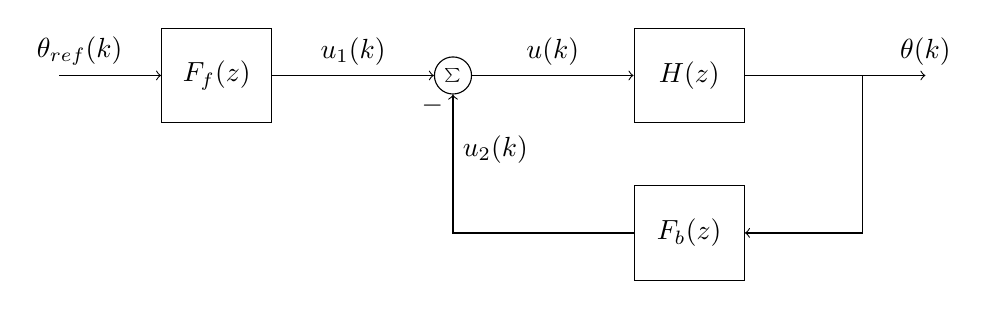
\begin{tikzpicture}
\tikzset{node distance=2cm, 
    block/.style={rectangle, draw, minimum height=12mm, minimum width=14mm},
    sumnode/.style={circle, draw, inner sep=2pt}        
}

  \node[coordinate] (input) {};
  \node[block, right of=input] (TR) {$F_f(z)$};
  \node[sumnode, right of=TR, node distance=30mm] (sum) {\tiny $\sum$};
  \node[block,right of=sum, node distance=30mm] (plant) {$H(z)$};
  %\node[sumnode, right of=plant, node distance=30mm] (sumdist) {$\sum$};
  %\node[coordinate, above of=sumdist, node distance=15mm] (dist) {};
  %\node[coordinate, right of=sumdist, node distance=15mm] (measure) {};
  \node[coordinate, right of=plant, node distance=30mm] (output) {};
  \node[coordinate, right of=plant, node distance=22mm] (measure) {};
  %\node[sumnode,below of=measure, node distance=25mm] (sumnoise) {$\sum$};
  %\node[coordinate, right of=sumnoise, node distance=15mm] (noise) {};
  \node[block,below of=plant, node distance=20mm] (SR) {$F_b(z)$};
  \draw[->] (input) -- node[above, pos=0.2] {$\theta_{ref}(k)$} (TR);
  \draw[->] (TR) -- node[above] {$u_1(k)$} (sum);
  \draw[->] (sum) -- node[above] {$u(k)$} (plant);
  \draw[->] (plant) -- node[at end, above] {$\theta(k)$} (output);
  \draw[->] (measure) |- (SR);
  \draw[->] (SR) -| (sum) node[right, pos=0.8] {$u_2(k)$} node[left, pos=0.96] {$-$};
\end{tikzpicture}
\end{center}
Usando \[U(z) = U_1(z) - U_2(z) = F_f(z)\Theta_{ref}(z) - F_b(z)\Theta(z), \quad \text{y}\]
\[ \Theta(z) = H(z)U(z), \quad \text{obtenemos} \]
\[ \Theta(z) = \underbrace{\frac{F_f(z)H(z)}{1 + F_b(z)H(z)}}_{H_c{z}} \Theta_{ref}(z). \]
\end{frame}

\begin{frame}[label={sec:org15ba77e}]{Estabilidad del sistem an lazo cerrado}
\[ \Theta(z) = \underbrace{\frac{F_f(z)H(z)}{1 + F_b(z)H(z)}}_{H_c{z}} \Theta_{ref}(z). \]

\begin{tcolorbox}
Estabilidad requiere que todos los polos del sistema, es decir las soluciones de la ecuación característica
\[ 1 + F_b(z)H(z) = 0\]
están en el interior del circulo unitario  del plano $z$.
\end{tcolorbox}
\end{frame}

\section{Ecuación característica}
\label{sec:orgbe4b919}

\section{Criterion de Nyquist para estabilidad - márgenes de estabilidad}
\label{sec:orge960397}

\begin{frame}[label={sec:orgf03a06b}]{Sinusoide entra - sinusoide sale}
\begin{center}
  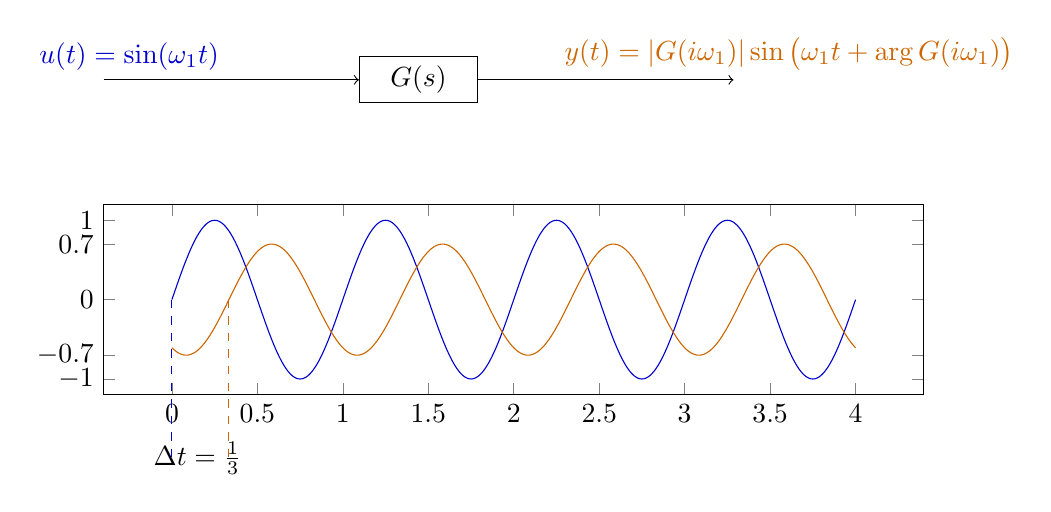
\begin{tikzpicture}[node distance=22mm, block/.style={rectangle, draw, minimum width=15mm}, sumnode/.style={circle, draw, inner sep=2pt}]

    \node[coordinate] (input) {};
    \node[block, right of=input, node distance=40mm] (plant)  {$G(s)$};
    \node[coordinate, right of=plant, node distance=40mm] (output) {};

    \draw[->] (input) -- node[above, pos=0.1, color=blue!80!black] {$u(t)=\sin(\omega_1 t)$} (plant);
    \draw[->] (plant) -- node[above, pos=0.3, anchor=south west, color=orange!80!black] {$y(t)=|G(i\omega_1)|\sin\big( \omega_1 t + \arg G(i\omega_1)\big)$} (output);


    \begin{axis}[
      yshift=-4cm,
      width=12cm,
      height=4cm,
      clip=false,
      ytick ={-1,-0.7, 0, 0.7, 1},
      ]
      \addplot[blue!80!black, no marks, domain=0:4, samples=600] {sin(360*x)};
      \addplot[orange!80!black, no marks, domain=0:4, samples=600] {0.7*sin(360*x - 120)};
      \draw[dashed, blue!80!black] (axis cs: 0, 0) -- (axis cs: 0, -2);
      \draw[dashed, orange!80!black] (axis cs: 0.333, 0) -- (axis cs: 0.333, -2);
      \node at (axis cs: 0.15, -2) {$\Delta t=\frac{1}{3}$};
    \end{axis}
  \end{tikzpicture}
  \end{center}
\(\omega_1 = \frac{2\pi}{T} = 2\pi\), \(|G(i\omega_1)| = 0.7\), \(\arg G(i\omega_1) = -\omega_1 \Delta t = -2\pi \frac{1}{3} = - \frac{2\pi}{3}\)
\end{frame}
\begin{frame}[label={sec:orgbd28666}]{Sinusoide entra - sinusoide sale}
\begin{center}
  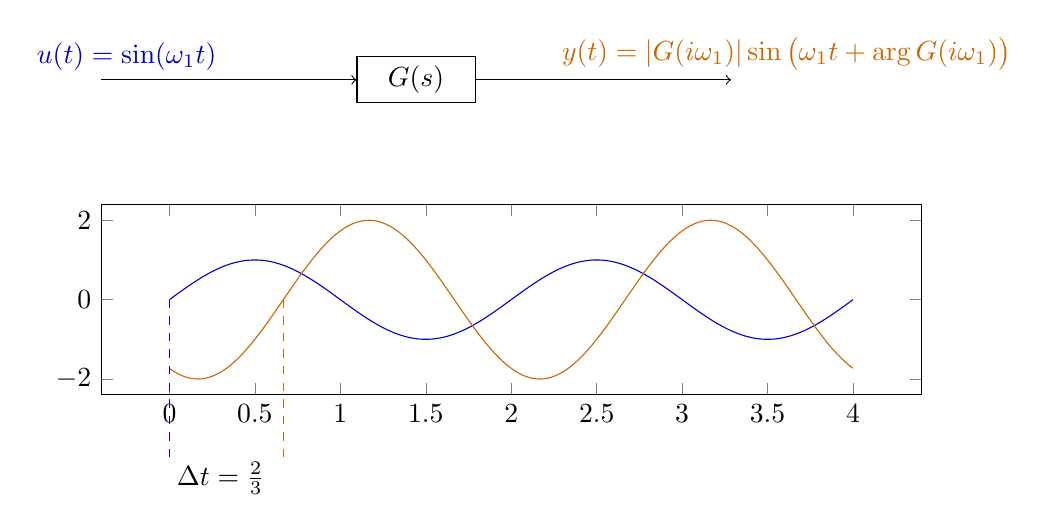
\begin{tikzpicture}[node distance=22mm, block/.style={rectangle, draw, minimum width=15mm}, sumnode/.style={circle, draw, inner sep=2pt}]

    \node[coordinate] (input) {};
    \node[block, right of=input, node distance=40mm] (plant)  {$G(s)$};
    \node[coordinate, right of=plant, node distance=40mm] (output) {};

    \draw[->] (input) -- node[above, pos=0.1, color=blue!80!black] {$u(t)=\sin(\omega_1 t)$} (plant);
    \draw[->] (plant) -- node[above, pos=0.3, anchor=south west, color=orange!80!black] {$y(t)=|G(i\omega_1)|\sin\big( \omega_1 t + \arg G(i\omega_1)\big)$} (output);


    \begin{axis}[
      yshift=-4cm,
      width=12cm,
      height=4cm,
      clip=false,
      %ytick ={-1,-0.7, 0, 0.7, 1},
      ]
      \addplot[blue!80!black, no marks, domain=0:4, samples=600] {sin(180*x)};
      \addplot[orange!80!black, no marks, domain=0:4, samples=600] {2*sin(180*x - 120)};
      \draw[dashed, blue!80!black] (axis cs: 0, 0) -- (axis cs: 0, -4);
      \draw[dashed, orange!80!black] (axis cs: 0.667, 0) -- (axis cs: 0.667, -4);
      \node at (axis cs: 0.3, -4.5) {$\Delta t=\frac{2}{3}$};
    \end{axis}
  \end{tikzpicture}
  \end{center}
\(\omega_1 = \frac{2\pi}{T} = \qquad\),   \(| G(i\omega_1)| = \qquad\),   \(\arg G(i\omega_1) = -\omega_1 \Delta t = \;\) 
\end{frame}

\begin{frame}[label={sec:org09f6340}]{Si el cambio de fase es \(\pi\)}
\(G_o(i\omega_1) = -1\), \(|G_o(i\omega_1)| = 1\), \(\arg G_o(i\omega_1) = -\pi\)

\begin{center}
  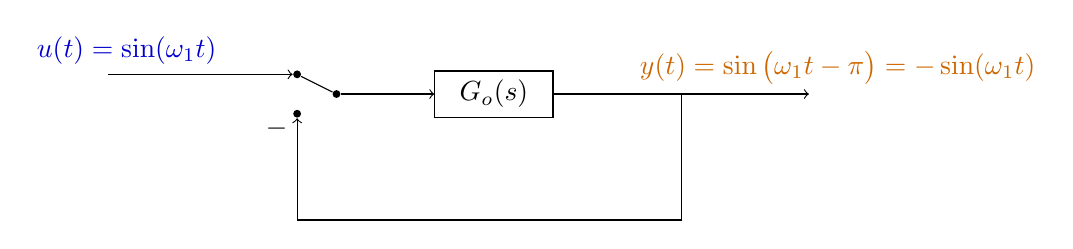
\begin{tikzpicture}[node distance=22mm, block/.style={rectangle, draw, minimum width=15mm}, sumnode/.style={circle, draw, inner sep=2pt}]

    \node[coordinate] (input) {};
    \node[circle, fill, inner sep=1pt, right of=input, node distance=24mm] (sum) {};
    \node[circle, fill, inner sep=1pt, below of=sum, node distance=5mm] (sum2) {};
    \node[coordinate, below of=sum, node distance=2.5mm] (summid) {};
    \node[circle, fill, inner sep=1pt, right of=summid, node distance=5mm] (sum3) {};
    \node[block, right of=sum3, node distance=20mm] (plant)  {$G_o(s)$};
    \node[coordinate, right of=plant, node distance=40mm] (output) {};

    \draw[->] (input) -- node[above, pos=0.1, color=blue!80!black] {$u(t)=\sin(\omega_1 t)$} (sum);
    \draw[->] (plant) -- node[coordinate, pos=0.5] (measure) {} node[above, pos=0.3, anchor=south west, color=orange!80!black] {$y(t)=\sin\big(\omega_1 t -\pi\big) = -\sin(\omega_1 t)$} (output);
    \draw[->] (sum3) -- node[above] {} (plant);
    \draw[->] (measure) -- ++(0,-16mm) -| node[pos=0.95, left] {$-$} (sum2);
    \draw (sum) to (sum3);
  \end{tikzpicture}
\end{center}
Función de transferencia del sistema de lazo cerrado: \(G_c(s) = \frac{G_o(s)}{1 + G_o(s)}\)
\begin{tcolorbox}
Queremos \[ 1 + G_o(i\omega) \neq 0, \quad \forall \omega \]
Si no, el sistema en lazo cerrado tendrá polos en el eje imaginario. 
\end{tcolorbox}
\end{frame}

\begin{frame}[label={sec:orgf3e9d56}]{Criterion (simplificado) de Nyquist en el plano \(s\)}
\begin{center}
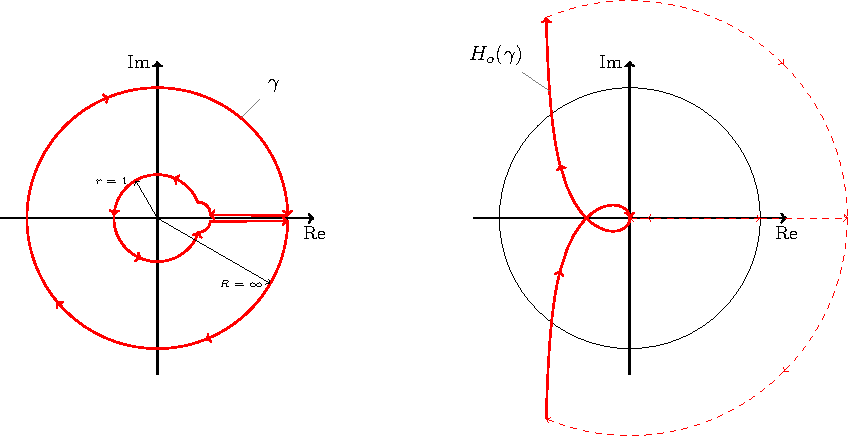
\includegraphics[width=0.65\linewidth]{../../figures/implane-nyquist-contour-map}
\end{center}
\begin{tcolorbox}
Si la gananzia del lazo abierto (\textit{loop gain}) $G_o(s)$ no tiene polos en el semiplano derecho (ningun polo inestable), entonces el sistem en lazo cerrado será estable si la curva de Nyquist \textbf{no rodea el punto \(s=-1\)}. El punto $s=-1$ debe quedarse al lado izquierdo (afuera) de la curva de Nyquist cuando "caminamos" a lo largo de la curva.
\end{tcolorbox}
\end{frame}

\begin{frame}[label={sec:org27af8ea}]{Márgenes de estabilidad relativa}
\begin{center}
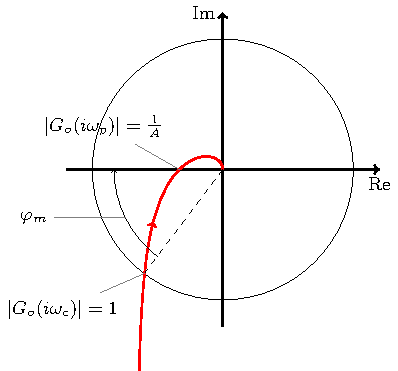
\includegraphics[width=0.38\linewidth]{../../figures/implane-nyquist-margins}
\end{center}
\begin{itemize}
\item Cross-over frequency: The frequency \(\omega_c\) for which \(|G_o(i\omega)| = 1\).
\item Phase margin: The angle \(\varphi_m\) to the negative real axis for the point where the Nyquist curve intersects the unit circle. \[\varphi_m = \arg G_o(i\omega_c) - (-180\degree) = \arg G_o(i\omega_c) + 180\degree\]
\end{itemize}
\end{frame}
\begin{frame}[label={sec:org0be6823}]{Márgenes de estabilidad relativa}
\begin{center}
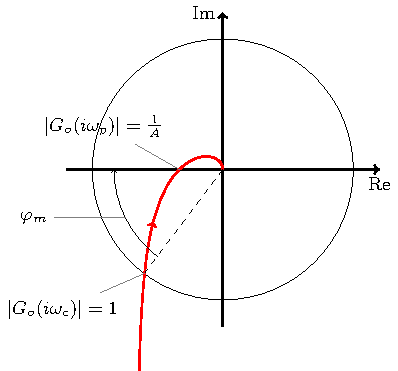
\includegraphics[width=0.38\linewidth]{../../figures/implane-nyquist-margins}
\end{center}
\begin{itemize}
\item phase-cross-over frequency: The frequency \(\omega_p\) for which \(\arg G_o(i\omega) = -180\degree\).
\item Gain margin: The gain \(K=A\) that would make the Nyquist curve of \(KG_o(i\omega h)\) go through the point \(-1 + i0\). This means that \[ |G_o(i\omega_p h| = \frac{1}{A}. \]
\end{itemize}
\end{frame}



\begin{frame}[label={sec:orgea3c68d}]{Efecto de muestreo y retención a los márgenes de estabilidad}
\[G(s) = \frac{1}{s^2 + 1.4s + 1} \quad \overset{h=0.4}{\longrightarrow} \quad H(z) = \frac{0.066z + 0.055}{z^2 - 1.450z + 0.571}\] 
\begin{center}
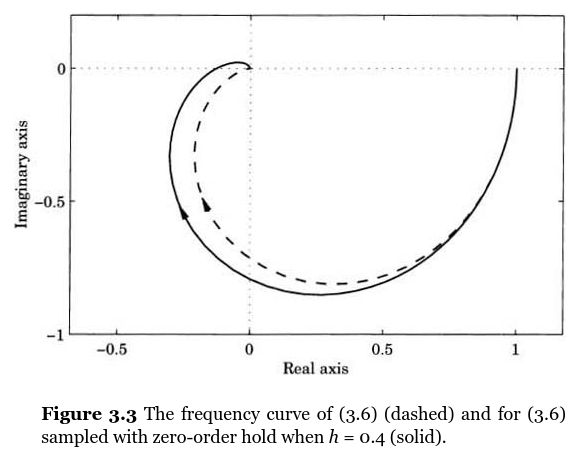
\includegraphics[width=0.6\linewidth]{../../figures/fig3-3.png}
\end{center}
\end{frame}
\begin{frame}[label={sec:org85cd3cd}]{Efecto de muestreo y retención a los márgenes de estabilidad}
\[G(s) = \frac{1}{s^2 + 1.4s + 1} \quad \overset{h=0.4}{\longrightarrow} \quad H(z) = \frac{0.066z + 0.055}{z^2 - 1.450z + 0.571}\] 
\begin{center}
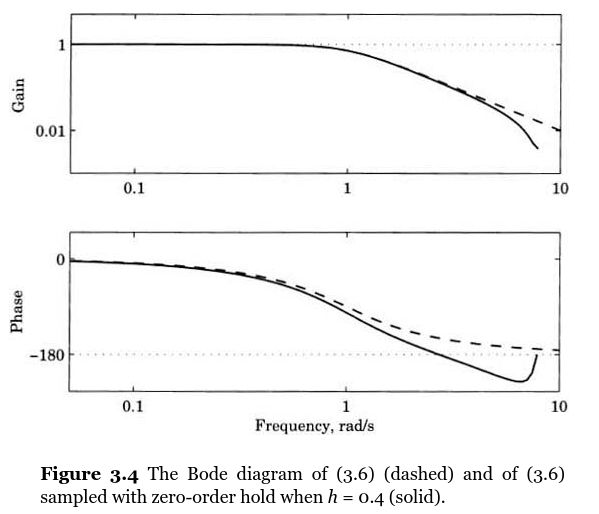
\includegraphics[width=0.5\linewidth]{../../figures/fig3-4.png}
\end{center}
\end{frame}

\begin{frame}[label={sec:orgf3d4807}]{Selección del tiempo de muestreo}
Se puede usar el cambio en el márgen de fase causada por el muestreo para determinar un tiempo de muestreo adecuado. Dado \(\omega_c\) y un máximo cambio negative en el márgen de fase \(\Delta\varphi \approx 5^\circ\; - \; 15^\circ \approx 0.09 \text{rad}\; - \; 0.26\text{rad}\) (una "regla de oro").

\begin{center}
  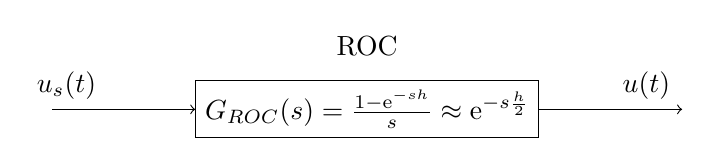
\begin{tikzpicture}[node distance=22mm, block/.style={rectangle, draw, minimum width=15mm}, sumnode/.style={circle, draw, inner sep=2pt}]

    \node[coordinate] (input) {};
    \node[block, right of=input, node distance=40mm] (plant)  {$G_{ROC}(s) = \frac{1 - \mathrm{e}^{-sh}}{s}\approx \mathrm{e}^{-s\frac{h}{2}}$};
    \node[coordinate, right of=plant, node distance=40mm] (output) {};

    \draw[->] (input) -- node[above, pos=0.1, ] {$u_s(t)$} (plant);
    \draw[->] (plant) -- node[above, near end,] {$u(t)$} (output);
    \node[above of=plant,  node distance=8mm] {ROC};
  \end{tikzpicture}
\end{center}
\[ \arg G_{ROC}(i\omega_c) \approx \arg \mathrm{e}^{i\omega_c \frac{h}{2}} = \omega_c \frac{h}{2} \approx 0.09 \text{rad}\; - \; 0.26\text{rad} \]

\alert{Actividad} Usa la \emph{regla de oro} arriba para calcular un tiempo de muestreo si \(\omega_c = \unit{20}{\rad\per\second}\) y \(\Delta\varphi = \unit{0.2}{\rad}\).
\end{frame}

\section{Jury's criterion}
\label{sec:org173bf3a}

\begin{frame}[label={sec:org3747fa0}]{El criterion de Jury}
\end{frame}
\begin{frame}[label={sec:org4d06787}]{Estabilidad para el control del brazo del disko duro}
\begin{center}
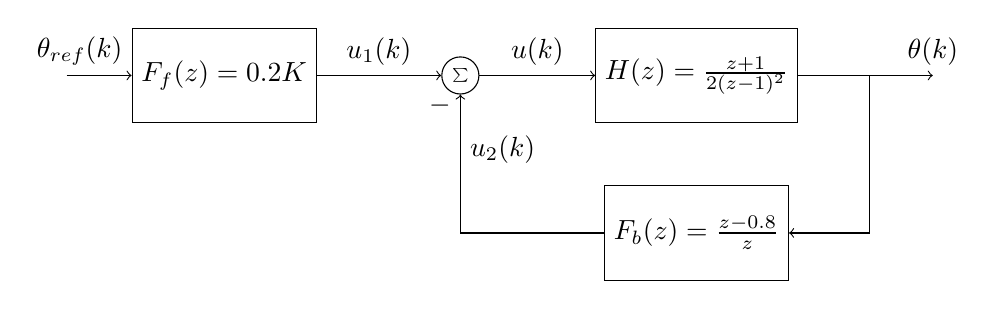
\begin{tikzpicture}
\tikzset{node distance=2cm, 
    block/.style={rectangle, draw, minimum height=12mm, minimum width=14mm},
    sumnode/.style={circle, draw, inner sep=2pt}        
}

  \node[coordinate] (input) {};
  \node[block, right of=input] (TR) {$F_f(z) = 0.2K$};
  \node[sumnode, right of=TR, node distance=30mm] (sum) {\tiny $\sum$};
  \node[block,right of=sum, node distance=30mm] (plant) {$H(z) = \frac{z+1}{2(z-1)^2}$};
  %\node[sumnode, right of=plant, node distance=30mm] (sumdist) {$\sum$};
  %\node[coordinate, above of=sumdist, node distance=15mm] (dist) {};
  %\node[coordinate, right of=sumdist, node distance=15mm] (measure) {};
  \node[coordinate, right of=plant, node distance=30mm] (output) {};
  \node[coordinate, right of=plant, node distance=22mm] (measure) {};
  %\node[sumnode,below of=measure, node distance=25mm] (sumnoise) {$\sum$};
  %\node[coordinate, right of=sumnoise, node distance=15mm] (noise) {};
  \node[block,below of=plant, node distance=20mm] (SR) {$F_b(z)=\frac{z-0.8}{z}$};
  \draw[->] (input) -- node[above, pos=0.2] {$\theta_{ref}(k)$} (TR);
  \draw[->] (TR) -- node[above] {$u_1(k)$} (sum);
  \draw[->] (sum) -- node[above] {$u(k)$} (plant);
  \draw[->] (plant) -- node[at end, above] {$\theta(k)$} (output);
  \draw[->] (measure) |- (SR);
  \draw[->] (SR) -| (sum) node[right, pos=0.8] {$u_2(k)$} node[left, pos=0.96] {$-$};
\end{tikzpicture}
\end{center}

\alert{Ecuación característica}
\begin{align*}
1 + H(z)F_b(z) &= 0\\
1 + \frac{z+1}{2(z-1)^2}K\frac{z-0.8}{z} &= 0\\
(z-1)^2z + \frac{K}{2}(z+1)(z-0.8) &= 0
\end{align*}
\end{frame}


\begin{frame}[label={sec:org72356d5}]{El método de Jury para analizar estabilidad}
Tenemos el polinomio característico
\[z^3 - 2z^2 + z + \frac{K}{2}(z^2 + 0.2z - 0.8)= z^3 + (0.5K-2)z^2 + (1+0.1K)z - 0.4K\]

\alert{El método de Jury se usa para analisar si un polynomio tiene todos sus raíces en el interior del círculo unitario}
\end{frame}

\begin{frame}[label={sec:org4f37738}]{El método de Jury para analizar estabilidad}
Es similar al método de Routh-Hurwitz de sistemas continuosos.

Considera el sistema
\[ H(z) = \frac{B(z)}{A(z)}. \] Es estable? Tenemos que investigar si los raíces del denominador están en el interior del círculo unitario.

La idea es investigar ciertas relaciónes algebraicas entre los coeficientes del polinomio \(A(z) = a_0z^n + a_1z^{n-1} + \cdots + a_n\).
\end{frame}

\begin{frame}[label={sec:orga4e2851}]{El método de Jury para analizar estabilidad}
Con \(A(z) = a_0z^n + a_1z^{n-1} + \cdots + a_n\), forma la tabla

\begin{center}
\begin{tabular}{llllll}
\(a_0\) & \(a_1\) & \(\cdots\) & \(a_{n-1}\) & \(a_n\) & \\
\(a_n\) & \(a_{n-1}\) & \(\cdots\) & \(a_1\) & \(a_0\) & \(\alpha_n =\frac{a_n}{a_0}\)\\
\hline
\(a_0^{n-1}\) & \(a_1^{n-1}\) & \(\cdots\) & \(a_{n-1}^{n-1}\) &  & \\
\(a_{n-1}^{n-1}\) & \(a_{n-1}^{n-1}\) & \(\cdots\) & \(a_0^{n-1}\) &  & \(\alpha_{n-1} =\frac{a_n^{n-1}}{a_0^{n-1}}\)\\
\hline
\(\vdots\) & \(\vdots\) & \(\vdots\) & \(\vdots\) & \(\vdots\) & \\
\hline
\(a_0^{0}\) & 0 & \(\cdots\) & 0 &  & \\
\end{tabular}
\end{center}

Las dos filas primeras son los coeficients de \(A(z)\). La tercera fila se obtiene eliminando el último elemento de la fila una: Multiplica fila 2 por \(\alpha_n = \frac{a_n}{a_0}\) y subtrae de la fila 1. Se repita el procedimiento hasta que solamente el primer elemento de la fila no es cero.
\end{frame}

\begin{frame}[label={sec:orgeace97f}]{El método de Jury para analizar estabilidad}
Con \(A(z) = a_0z^n + a_1z^{n-1} + \cdots + a_n\), forma la tabla

El criterión dice que todos los raíces de \(A(z)\) están en el interior del circulo unitario, sí, y solo sí todos los elementos \(a_0^k\) el el primer columno tienen el mismo signo. 

Hay pruebas preliminares de estabilidad que podemos utilizar:
\begin{enumerate}
\item \(A(1) > 0\)
\item \((-1)^nA(-1) > 0\)
\item \(|a_0^k| > |a_k^k|\)
\end{enumerate}
\end{frame}


\begin{frame}[label={sec:org35d3afe}]{Ejemplo - control del brazo del disko duro}
Polinomio característico \[ A(z) = z^3 + (0.5K-2)z^2 + (1+0.1K)z - 0.4K\]
\begin{center}
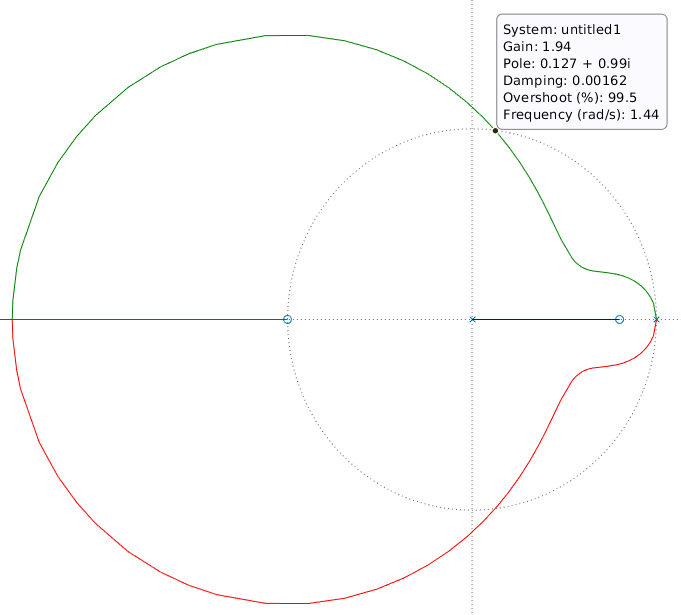
\includegraphics[width=0.5\linewidth]{../../figures/diskdrive-lead-discrete-rlocus.png}
\end{center}
\end{frame}

\begin{frame}[label={sec:org83da073}]{Ejemplo - Método de Jury}
Polinomio característico \[ A(z) = z^3 + (0.5K-2)z^2 + (1+0.1K)z - 0.4K\]

Aplica las pruebas preliminares 1 y 2:
\begin{enumerate}
\item \(A(1) > 0\)
\item \((-1)^nA(-1) > 0\)
\end{enumerate}
\end{frame}

\begin{frame}[label={sec:orgb9951a1}]{Ejemplo - Método de Jury}
Polinomio característico \[ A(z) = z^3 + (0.5K-2)z^2 + (1+0.1K)z - 0.4K\]

Aplica las pruebas preliminares 1 y 2:
\begin{enumerate}
\item \(A(1) > 0\)
\item \((-1)^nA(-1) > 0\)
\begin{align}
(-1)^3A(-1) &= -\left((-1)^3 + (0.5K-2)(-1)^2 + (1+0.1K)(-1) - 0.4K \right)\\
 &= 1-(0.5K-2) +(1+0.1K) + 0.4K > 0\\
 &=4 >0, \quad \text{Holds for all \(K\)}
 \end{align}
\end{enumerate}


\alert{Actividad} Aplica prueba 1!
\end{frame}

\begin{frame}[label={sec:org1e53840}]{Ejemplo - Método de Jury}
Tenemos el polinomio característico \(e A(z) = z^3 + (0.5K-2)z^2 + (1+0.1K)z - 0.4K\). La tabla sería

\begin{center}
\begin{tabular}{lllr}
1 & \(0.5K - 2\) & \(0.1K + 1\) & \(-0.4K\)\\
\(-0.4K\) & \(0.1K + 1\) & \(0.5K - 2\) & 1\\
\(-0.16K^2 + 1\) & \(0.04K^2 + 0.9K - 2\) & \(0.2K^2 - 0.7K + 1\) & 0\\
\(0.2K^2 - 0.7K + 1\) & \(0.04K^2 + 0.9K - 2\) & \(-0.16K^2 + 1\) & 0\\
\(\frac{K(0.0144K^3 - 0.28K^2 + 1.21K - 1.4)}{0.16K^2 - 1.0}\) & \(\frac{K(0.0144K^3 + 0.296K^2 - 1.35K + 1.4)}{0.16K^2 - 1.0}\) & 0 & 0\\
\(\frac{K(0.0144K^3 + 0.296K^2 - 1.35K + 1.4)}{0.16K^2 - 1.0}\) & \(\frac{K(0.0144K^3 - 0.28K^2 + 1.21K - 1.4)}{0.16K^2 - 1.0}\) & 0 & 0\\
\end{tabular}
\end{center}

Para estabilidad necesitamos
\begin{align*}
 -0.16K^2 + 1 &> 0 \\
\frac{K(0.0144K^3 - 0.28K^2 + 1.21K - 1.4)}{0.16K^2 - 1} &> 0
\end{align*}
\end{frame}

\begin{frame}[label={sec:orge13e3af}]{Ejemplo - Método de Jury}
Para estabilidad necesitamos
\[ -0.16K^2 + 1 > 0 \quad \Rightarrow \quad K < \sqrt{\frac{1}{0.16}} = 2.5\]
Asumiendo  \(0<K<2.5\)
\[ 0.0144K^3 - 0.28K^2 + 1.21K - 1.4 < 0 \quad \Rightarrow \quad x < \frac{35}{18} \approx 1.94\] 

\begin{tcolorbox}
 El sistema en lazo cerrado será estable si \[ 0 < K < 1.94\]
\end{tcolorbox}
\end{frame}

\begin{frame}[label={sec:orgb07a6a3}]{Ejercicio - estabilidad de sistemas de segunda orden}
Polinomio característico \[A(z) = z^2 + a_1z + a_2\]

\alert{Actividad} Forma la tabla de Jury, y determina los valores de \(a\) y \(b\) que da raíces dentro del circulo unitario.

Puedes utilizar 
\[ 1-a_2^2 - \frac{a_1^2(1-a_2)}{1+a_2} = \frac{(1-a^2)(1+a_2) - a_1^2(1-a_2)}{1+a_2} = \frac{1-a_2}{1+a_2}\big((1+a_2)^2 - a_1^2\big)\]
\end{frame}

\begin{frame}[label={sec:orgf62d041}]{Ejercicio - Solución}
Polinomio característico \[A(z) = z^2 + a_1z + a_2\]

\begin{center}
\begin{tabular}{llr}
1 & \(a_1\) & \(a_2\)\\
\(a_2\) & \(a_1\) & 1\\
\(1 - a_2^2\) & \(a_1(1-a_2\) & 0\\
\(a_1(1-a_2\) & \(1 - a_2^2\) & 0\\
\(1-a_2^2 - \frac{a_1^2(1-a_2)}{1+a_2}\) & 0 & \\
\end{tabular}
\end{center}

Los raíces van a estar adentro del circulo unitario si
\begin{align*}
  1 - a_2^2 &> 0 \quad \Rightarrow \quad -1 < a_2 < 1\\
  \frac{1-a_2}{1+a_2} \big((1+a_2)^2 - a_1^2\big) &> 0\\
\end{align*}
\end{frame}

\begin{frame}[label={sec:org418c724}]{Ejercicio - Solución}
   Con \(-1 < a_2 < 1\) la fraccion en 
   \[\frac{1-a_2}{1+a_2} \big((1+a_2)^2 - a_1^2\big) > 0\]
   siempre va a ser positiva.
   \[(1+a_2)^2 - a_1^2 > 0 \quad \Rightarrow \quad \begin{cases} 1+a_2 > a_1, & a_1 > 0,\\ 1 + a_2 > -a_1, & a_1 < 0 \end{cases}. \]
Los raíces del polinomio \(A(z) = z^2 + a_1z + a_2\) están adentro del circulo unitario si
\begin{align*}
a_1 &< 1\\
a_2 &> -1+a_1\\
a_2 &> -1 - a_1
\end{align*}
\end{frame}

\begin{frame}[label={sec:org09056ca}]{Ejercicio - graficar}
\begin{columns}
\begin{column}{0.5\columnwidth}
Los raíces del polinomio \(A(z) = z^2 + a_1z + a_2\) están adentro del circulo unitario si
\begin{align*}
a_1 &< 1\\
a_2 &> -1+a_1\\
a_2 &> -1 - a_1
\end{align*}

\alert{Dibuja la region definida por las inequalidades}
\end{column}
\begin{column}{0.5\columnwidth}
\begin{center}
  \begin{tikzpicture}[scale=0.8]
    \draw[->] (-4,0) -- (4,0) node[below] {$a_1$};
    \draw[->] (0,-3) -- (0,3) node[left] {$a_2$};
    \draw (0.1,2) -- (-0.1, 2) node[left] {1};
    \draw (0.1,-2) -- (-0.1, -2) node[left] {-1};
  \end{tikzpicture}
\end{center}
\end{column}
\end{columns}
\end{frame}
\end{document}